% Abstract template for Physics Days 2022
\documentclass[12pt, a4paper]{article}
\usepackage{fp2022}

\usepackage{graphicx}
\usepackage{caption}
\usepackage{mwe}

\usepackage{subcaption}

\begin{document}

%%%%%%%%%%%%%%%%%%%%%%%%%%%%%%%%%%%%%%%%%%%%%%%%%%%%%%%%%%%%%%%%%%%%%%%%%%%%%%%%
% Header 
%%%%%%%%%%%%%%%%%%%%%%%%%%%%%%%%%%%%%%%%%%%%%%%%%%%%%%%%%%%%%%%%%%%%%%%%%%%%%%%%


% Title in capital letters
\title{Multi-fidelity machine learning to accelerate materials research}
% MT: Combining multi-fidelity simulations for materials research - is this too simple?

% List of authors with the presenting authors name underlined
{\underline{M.~Kuchelmeister}\textsuperscript{1}, J.~Löfgren\textsuperscript{1},
M.~Todorović\textsuperscript{2}, and P.~Rinke\textsuperscript{1}}

% Affiliations
{\textsuperscript{1}\em Department of Applied Physics, Aalto University}

{\textsuperscript{2}\em Department of Mechanical and Materials Engineering, University of Turku}

% Presenting authors email
email: manuel.kuchelmeister@aalto.fi

% Extra space after header
\vspace{2\baselineskip}

%%%%%%%%%%%%%%%%%%%%%%%%%%%%%%%%%%%%%%%%%%%%%%%%%%%%%%%%%%%%%%%%%%%%%%%%%%%%%%%%
% Main text
%%%%%%%%%%%%%%%%%%%%%%%%%%%%%%%%%%%%%%%%%%%%%%%%%%%%%%%%%%%%%%%%%%%%%%%%%%%%%%%%

The computational optimization and exploration of materials is a challenging task,
due to the high dimensionality of the search space and the high cost of accurate
quantum mechanical calculations. To reduce the number of costly calculations,
the Bayesian Optimization Structure Search (BOSS)~\cite{BOSS} has been developed.
BOSS combines sample-efficient active learning with Gaussian process regression.

We here present a multi-fidelity approach (Fig.~\ref{fig:tl_with_alanine}a) that
can reduce the number of costly, accurate calculations even further by
incorporating information from inexpensive but less accurate calculations.
We implemented the intrinsic model of coregionalization~\cite{ICM} method
into BOSS to sample data from multiple atomistic calculations
based on quantum chemistry (Gaussian 16, using CCSD(T)), density-functional theory 
(FHI-aims, using a PBE exchange-correlation functional) and force fields (AMBER18). 
Multi-fidelity BOSS is initialized with lower-fidelity data 
and continues to sample only higher-fidelity calculations, maintaining CCSD(T) 
accuracy for the global minimum inference.

We tested our multi-fidelity model on 4D alanine conformer search 
(Fig.~\ref{fig:tl_with_alanine}b).
The efficiency of our approach is measured by computational 
cost in CPU hours, comparing runs with and without lower-fidelity (LF) data 
(Fig.~\ref{fig:tl_with_alanine}c). We were able to reduce the computational
cost for a CCSD(T) run, when using DFT as LF data, by about 70\%. 
We found that the efficiency of the ICM model depends on both the correlation
and computational cost difference between the fidelities, as well as the
number of LF data. Our test serves as a first benchmark for the great
potential that multi-fidelity learning can have to reduce expensive 
structure-search problems.

\begin{figure}[h]
\centering
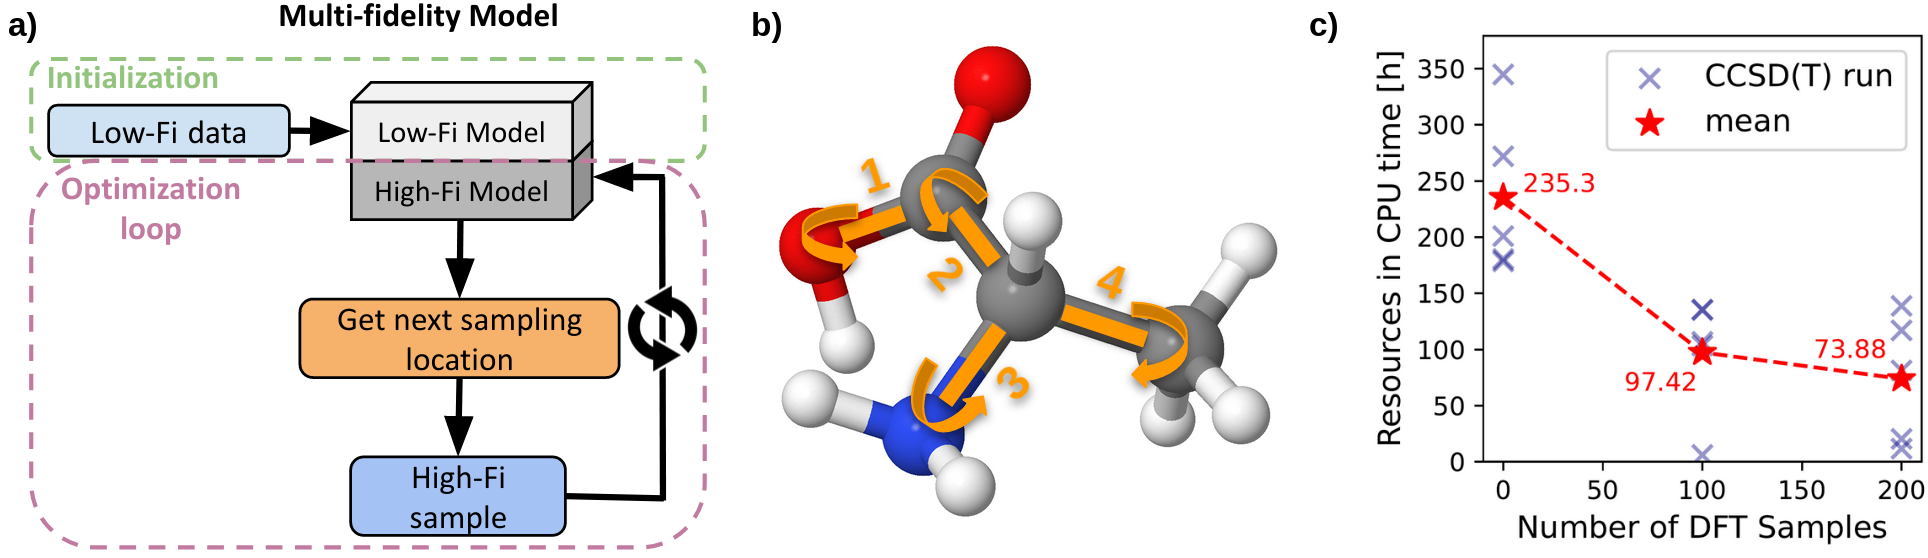
\includegraphics[width=\textwidth]{model_alanine_results.png}
\caption{a) Multi-fidelity BOSS framework. b) Atomistic model for the 4D alanine conformer search. 
c) Reduction in computational cost for CCSD(T) structure search with DFT as LF data.}
\label{fig:tl_with_alanine}
\end{figure}

%%%%%%%%%%%%%%%%%%%%%%%%%%%%%%%%%%%%%%%%%%%%%%%%%%%%%%%%%%%%%%%%%%%%%%%%%%%%%%%%
% Bibliography
%%%%%%%%%%%%%%%%%%%%%%%%%%%%%%%%%%%%%%%%%%%%%%%%%%%%%%%%%%%%%%%%%%%%%%%%%%%%%%%%

% Extra space after main text
\vspace{2\baselineskip}

\begin{thebibliography}{9}
\bibitem{BOSS} M.~Todorović, M.~U.~Gutmann, J.~Corander, and P.~Rinke, {\it npj Comput. Mater.} {\bf 5}, 35 (2019).
\bibitem{ICM} E.V.~Bonilla et al., {\it Advances in Neural Information Processing Systems} {pp.153-160} (2007).

\end{thebibliography}

\end{document}

